\chapter{Simulador}

% Que (es lo que deberia hacer) hace el simulador en la U
El simulador de vuelo del laboratorio de técnicas aeroespaciales es una herramienta muy útil para los alumnos de la universidad, otorgando una primera aproximación a los procedimientos necesarios para ejecutar un vuelo, y permite familiarizarse con los conceptos teóricos que se ven en clases de una manera práctica.

% Que hace el simulador en el PIA
Durante los años varios alumnos han trabajado con el equipo haciendo mejoras o investigación y es la forma en la que se ha mantenido el simulador operativo hasta hoy. Al estar relacionado el principal objetivo de este proyecto de ingeniería con el simulador, se hace notar la oportunidad de trabajar sobre el simulador en sí y llevar a cabo el proceso de su actualización con mejores componentes que están disponibles en el laboratorio, pero que aún no están instalados.

% Introducción a que se ve en el capitulo
En este capítulo se describe el proceso de actualización del equipo del simulador en hardware y software como está descrito en la metodología, los problemas que surgieron y el diseño final, comenzando por la caracterización del simulador en su condición inicial.

\section{Configuración inicial}

% Resumen hardware y software
El equipo consiste en 3 computadores conectados a 7 pantallas con una disposición de 5 pantallas abarcando el campo de visión horizontal y 2 pantallas auxiliares para mostrar instrumentos del panel, periféricos de control similares a los encontrados a una avioneta Cessna 172 \cite{saitek}, sistema de sonido y red local con router (\ref{fig:sim1}). El computador principal cuenta con Windows 10, procesador Intel i7 de tercera generación y tarjeta gráfica NVIDIA GTX 1060 (\ref{fig:sim2}), los dos computadores secundarios tienen Windows 7 y prestaciones mucho más bajas, pero suficientes para ejecutar X-Plane 9.

\begin{figure}[h]
	\centering
	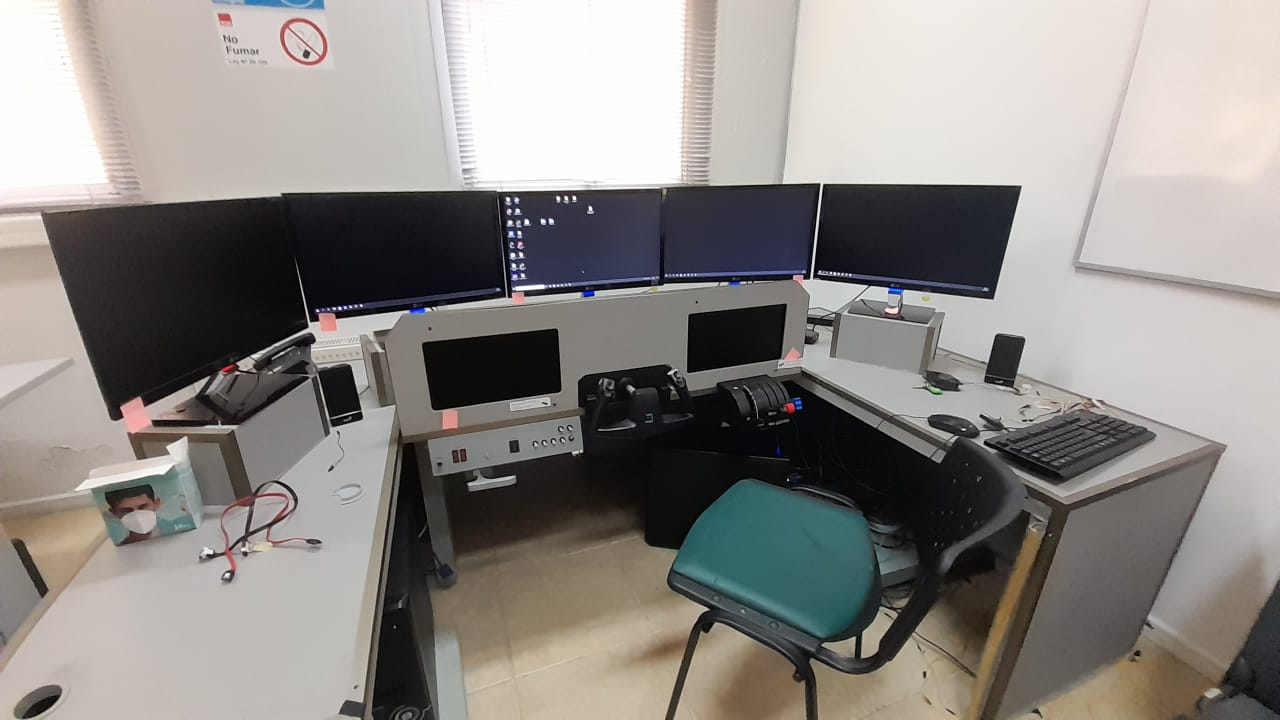
\includegraphics{sim1.jpeg}
	\caption{Simulador de vuelo con configuración original}
	\label{fig:sim1}
\end{figure}

\begin{figure}[h]
	\centering
	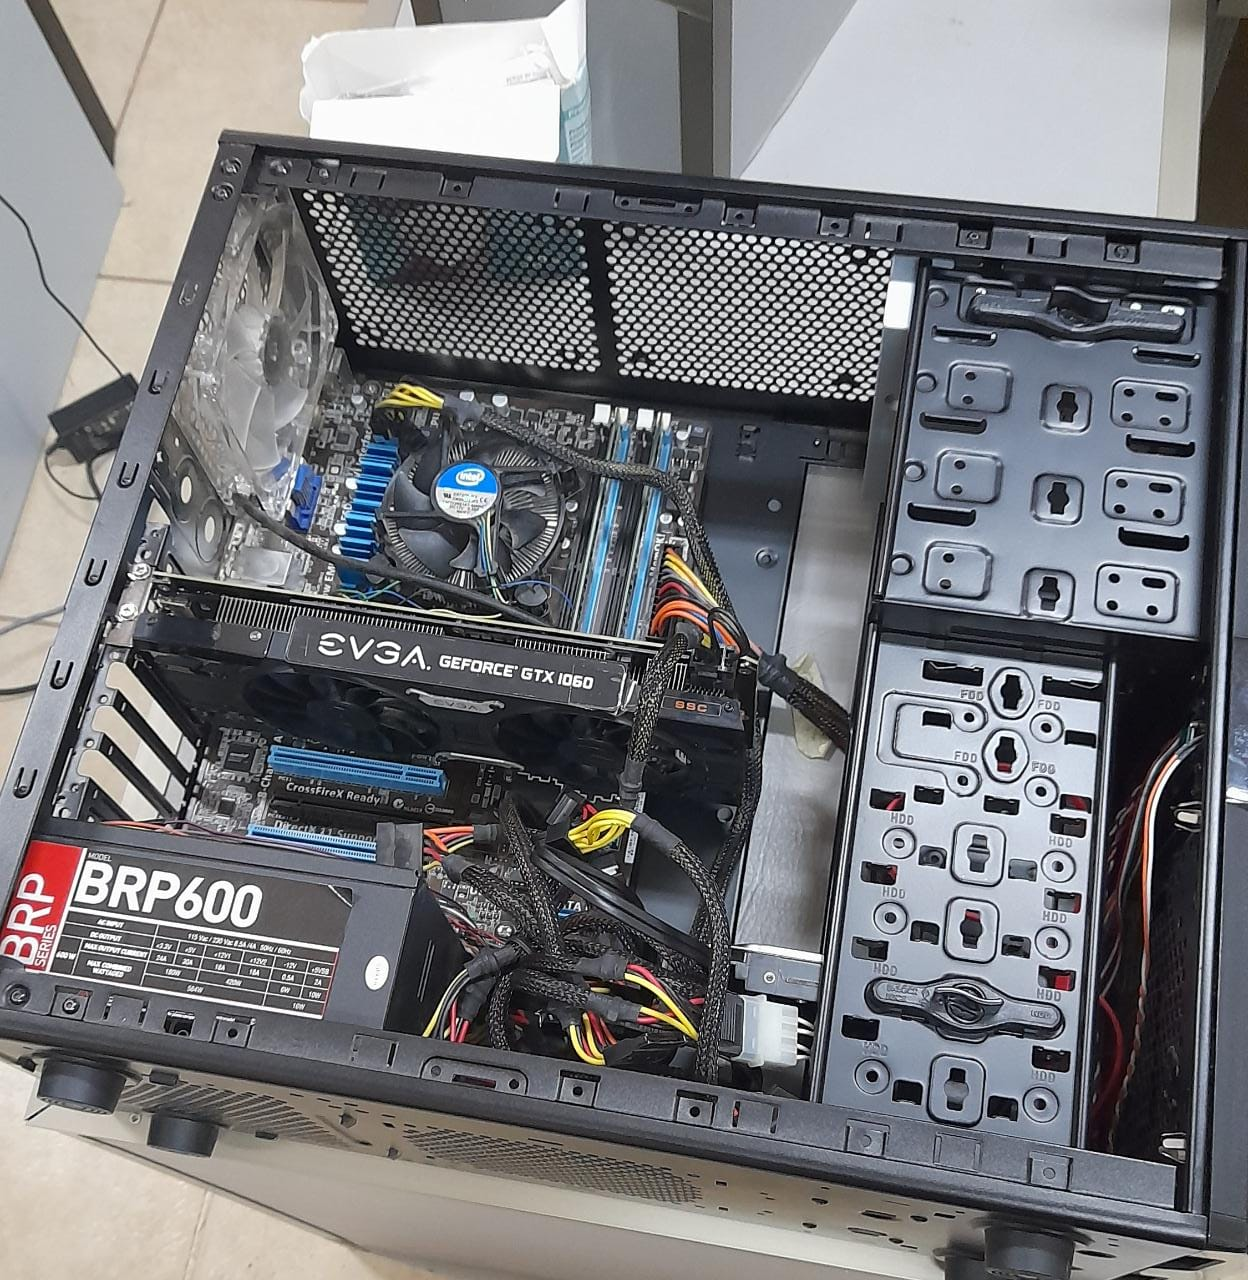
\includegraphics{sim2.jpeg}
	\caption{Computador principal con configuración original}
	\label{fig:sim2}
\end{figure}

% Como funciona X-Plane 9
Cada computador corre una instancia de X-Plane 9, el principal dirige la simulación, recibe la entrada de los controles y envía el estado de la simulación a los computadores secundarios por medio de la red local, los que replican el estado y actúan como extensión del campo de visión y despliegue del panel de instrumentos, todo configurado de acuerdo a las instrucciones del manual de usuario de X-Plane 9 \cite{manual9}.

\section{Alternativas de diseño}

% Que me pidieron y el problema con eso
Se solicita instalar dos componentes nuevos con el objetivo de ejecutar X-Plane 10 y posiblemente simuladores más recientes en el futuro, los cuales son una tarjeta gráfica NVIDIA GTX 1080 y una fuente de poder de 700 W. Considerando la configuración inicial del simulador y los objetivos, la instalación de los nuevos componentes no es un tema de solo reemplazar los antiguos, ya que los computadores secundarios seguirán obsoletos y limitados a X-Plane 9.

\subsection{Dos computadores}

% Alternativa inmediata
Una solución plausible es actualizar y reemplazar los componentes en el computador principal, el mejor de los secundarios actualizarlo con los componentes sobrantes (GTX 1060 y fuente) y descartar el tercer computador. Es inmediatamente la solución con menos complicaciones y (sin mencionar algunos detalles) compatible con la configuración de X-Plane ya implementada y descrita en los manuales, sin embargo tiene muchos problemas que surgirán a futuro.

% Por qué insistí tanto con no hacer eso
% El rendimiento y futuras actualizaciones
En rendimiento la GTX 1080 y 1060 soportan con creces X-Plane 10 (que no es mucho más exigente que X-Plane 9 gráficamente), pero el procesador de todos los computadores del simulador también requiere actualización, la tercera generación de Intel salió en 2012 y con nuevo software como X-Plane 12 esta empieza a mostrar sus limitaciones, el tener 2 computadores implica que en futuras actualizaciones se deban comprar el doble de componentes, los que probablemente solo cumplan con los requisitos mínimos de los simuladores nuevos, en vez de actualizar solo un computador con todo el presupuesto y asegurarse que podrá ejecutar el software de sobra.

% Complejo de configurar
Dos o más computadores requieren múltiples instalaciones del software de simulación (que para el caso de X-Plane implica comprar más licencias \cite{licencias}), configuración para la ejecución automática del software en cada computador si no se quiere tener que usar múltiples periféricos, o implementar soluciones para conectar periféricos a múltiples computadores, configurar una red local que asigne una IP estática distinta a cada computador para la posterior sincronización del software de simulación, si es que estos la soportan como X-Plane. Estos detalles y otros no mencionados significan mayor complejidad para trabajar en el simulador o poner en marcha nuevo software en el futuro.

\subsection{Un computador}

% Ventajas de solo un computador
En vista de los problemas recién mencionados, se evalúa la opción de usar solo un computador asignándole los mejores componentes disponibles, lo que elimina gran parte de las complicaciones de tener dos o más, pero que aún cumpla con los objetivos inmediatos. Implementar la configuración existente del simulador es fácil, por ejemplo si antes se tenían 3 instancias de X-Plane en computadores distintos ahora se pueden tener abiertas 3 instancias, pero en solo un computador con múltiples pantallas, claro que hacer eso es posible una vez puesto el hardware en marcha donde debido a las circunstancias surgen complicaciones.

\subsection{Múltiples pantallas}

% Contando cuantas salidas de video tenemos
No se pueden conectar 7 pantallas a una sola tarjeta de video, la GTX 1080 y GTX 1060 cada una permite hasta 4 monitores, el procesador Intel permite hasta 3 salidas de video con sus gráficos integrados \cite{i7-3770k}, pero la placa madre tiene solo dos salidas, una digital y una análoga. Existen adaptadores USB a HDMI que habilitan más salidas de video, pero la información que existe de ellos es muy variada, hay reportes de que estos adaptadores pueden reducir el rendimiento además de que cuestan dinero y no se puede asegurar que vayan a ser compatibles.

% 7 Pantallas usando solo los recursos disponibles en el laboratorio
Usando solo el material disponible en el laboratorio se decide por conectar ambas tarjetas de video simultáneamente al computador habilitando hasta 10 salidas, 8 desde las GPU y 2 de los gráficos integrados del procesador. Esto puede suponer un riesgo de recalentamiento, pero se esperará a ver con el tiempo si esto resulta en un problema a largo plazo, en caso de altas temperaturas se confía en que las unidades de procesamiento incluyen sensores que apagan el sistema antes de cualquier situación peligrosa para evitar daños.

% Crisis energética
Ambas tarjetas de video además de la interfaz PCI con la placa madre requieren ser conectadas directamente a la fuente de poder con cables de 6 y 8 pines dedicados para funcionar. La nueva fuente de poder no cuenta con los suficientes cables para ambas GPU, se podría comprar o fabricar un cable splitter para lograr conectar todo, pero supone mucho riesgo de recalentamiento por la calidad del splitter y la cantidad de energía que va a transmitir, la nueva fuente no está diseñada para eso.  

% Ventajas y desventajas
Usar dos fuentes de poder asegura que se cuenta con suficiente energía para alimentar ambas tarjetas de video sin riesgo a recalentamiento de cables, no se necesitan modificar internamente los componentes, puesto que aun en esta configuración están trabajando dentro de los parámetros establecidos por los fabricantes.

\section{Configuración final}

La nueva configuración consiste en reducir la cantidad de computadores de tres a solo uno, el cual en el futuro pueda ser actualizado con un buen procesador para ejecutar simuladores modernos como Flight Simulator 2020 o X-Plane 12. Además reduciendo la complejidad de tener que preparar múltiples computadores a solo tener que configurar en uno el software, donde en los casos que no exista soporte oficial para tantas pantallas (como en X-Plane 9 y 10) se pueden preparar scripts que abran múltiples instancias del simulador que repliquen la antigua configuración.

\subsection{Hardware}

% Instalación de nuevos componentes y problema a resolver
Se instalan los nuevos componentes al computador principal y se prueba que funcionen correctamente, las unidades de procesamiento del equipo en este punto son su procesador Intel i7-3770k y una tarjeta gráfica NVIDIA GTX 1080. Con esta configuración se ve limitada la cantidad de salidas de video disponibles como fue descrito previamente, por lo que se procede a realizar pruebas del funcionamiento del equipo al agregarse la tarjeta GTX 1060 y una segunda fuente.

% Pruebas de la solución y resultado
Con la segunda tarjeta gráfica conectada al puerto PCI disponible, se prepara la antigua fuente de poder para un encendido manual \cite{psumanual} y se conecta para alimentar la GTX 1060, por HDMI se conecta una quinta pantalla al equipo el cual se enciende para comprobar su funcionamiento. Las pruebas son un éxito (\ref{fig:sim3}) y se decide por instalar la segunda fuente dentro del gabinete (\ref{fig:sim4}).

\begin{figure}[h]
	\centering
	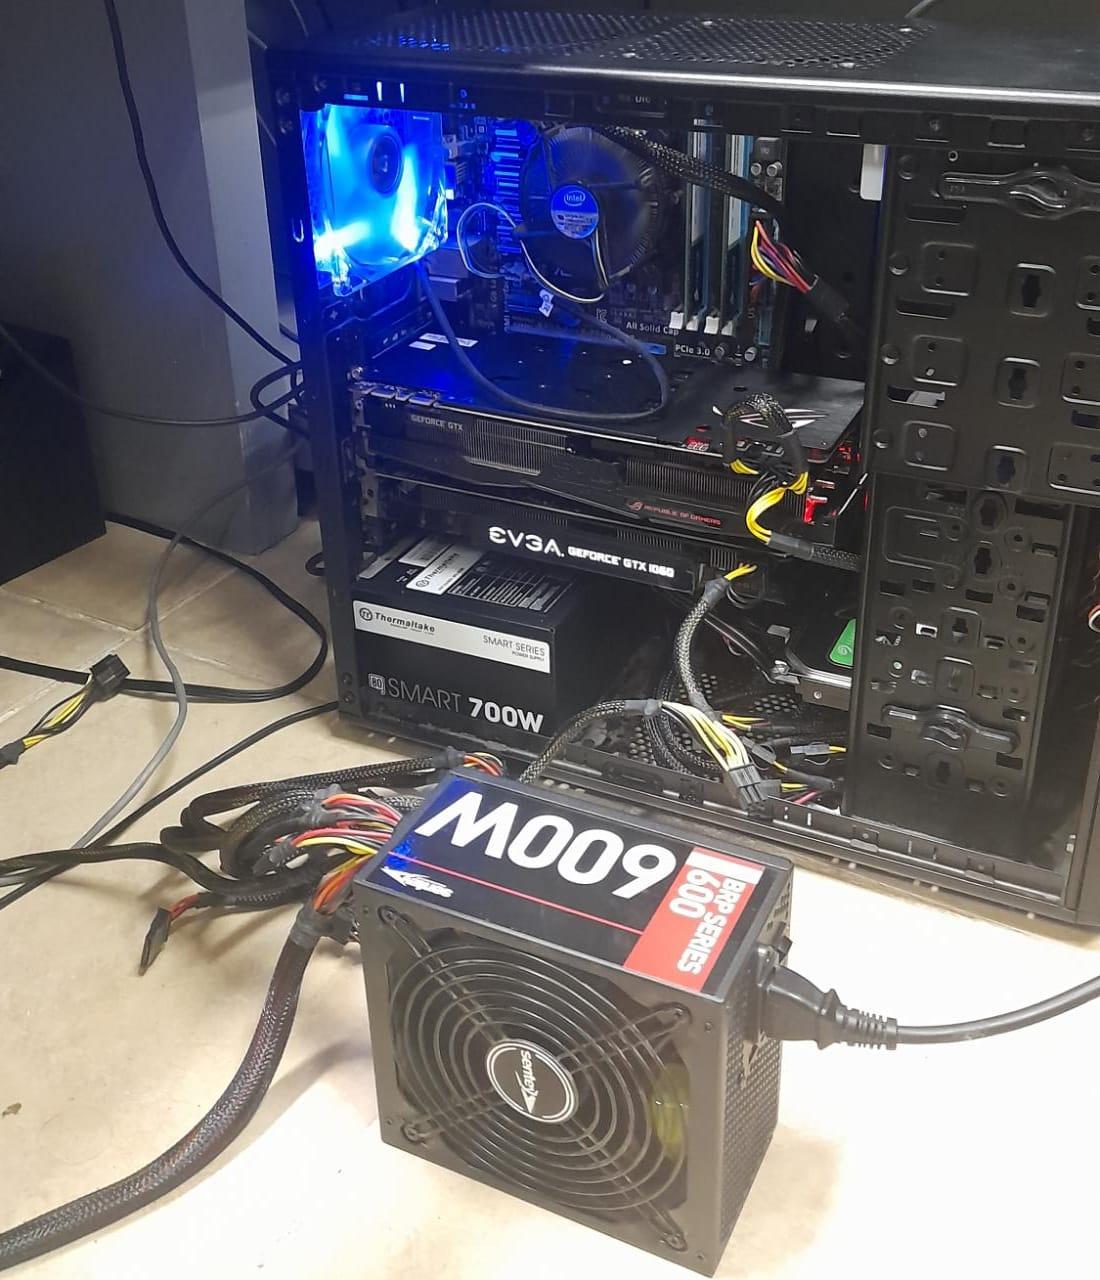
\includegraphics{sim3.jpeg}
	\caption{Prueba de encendido con segunda fuente de poder}
	\label{fig:sim3}
\end{figure}

\begin{figure}[h]
	\centering
	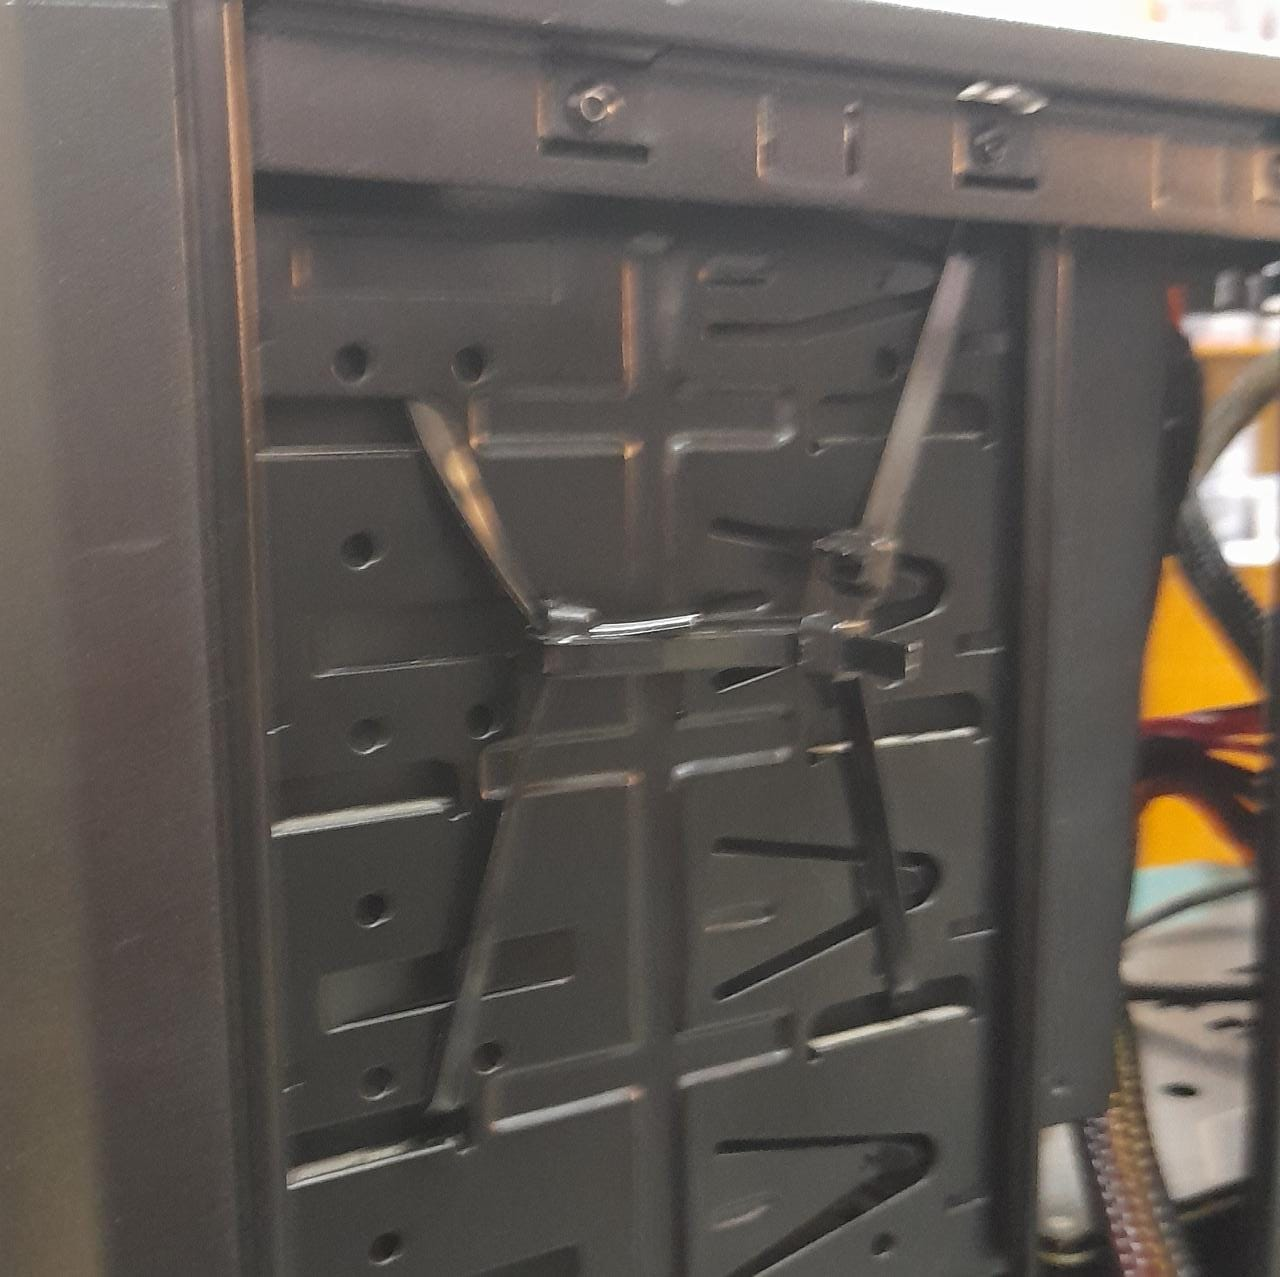
\includegraphics{sim4.jpeg}
	\caption{Instalación de segunda fuente con amarras plásticas}
	\label{fig:sim4}
\end{figure}

% Problema de sincronización y compra del sincronizador
Al no estar conectada directamente a la placa madre, la segunda fuente de poder necesita ser encendida y apagada manualmente al mismo tiempo que el computador, para resolver este problema se compra un dispositivo que sincroniza el encendido de la fuente auxiliar por medio de un relé (\ref{fig:sim5}).

\begin{figure}[h]
	\centering
	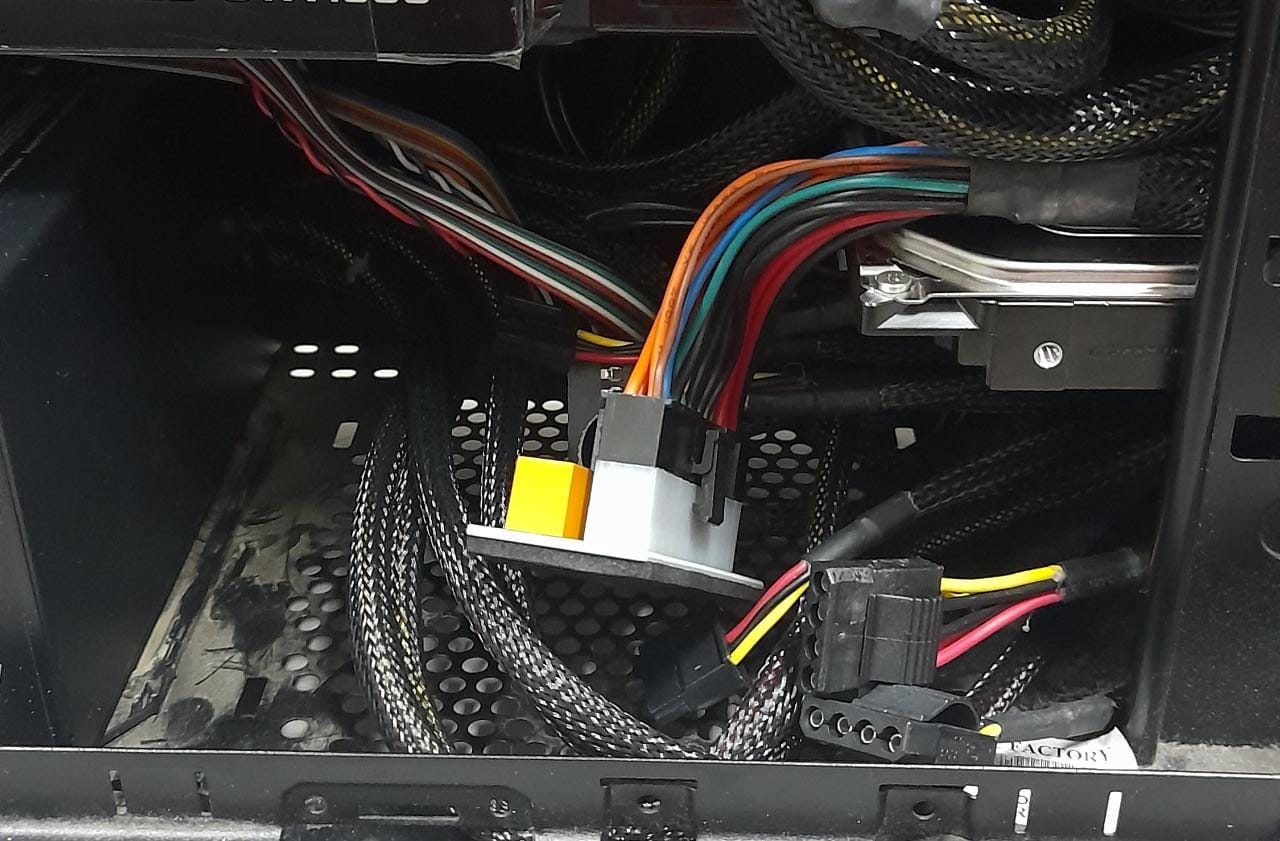
\includegraphics{sim5.jpeg}
	\caption{Dispositivo sincronizador de fuentes}
	\label{fig:sim5}
\end{figure}

% Configuración final de hardware
Finalmente se conectan todas las pantallas al equipo, terminando el proceso de actualización (\ref{fig:sim6}) y dando paso a comenzar la configuración del software de simulación. Los componentes principales del computador por el momento son el procesador Intel i7-3370k, dos tarjetas gráficas NVIDIA GTX 1080 y NVIDIA GTX 1060, y se espera que se introduzca en el futuro un mejor procesador que permita ejecutar software de simulación actual como Microsoft Flight Simulator 2020 y X-Plane 12.

\begin{figure}[h]
	\centering
	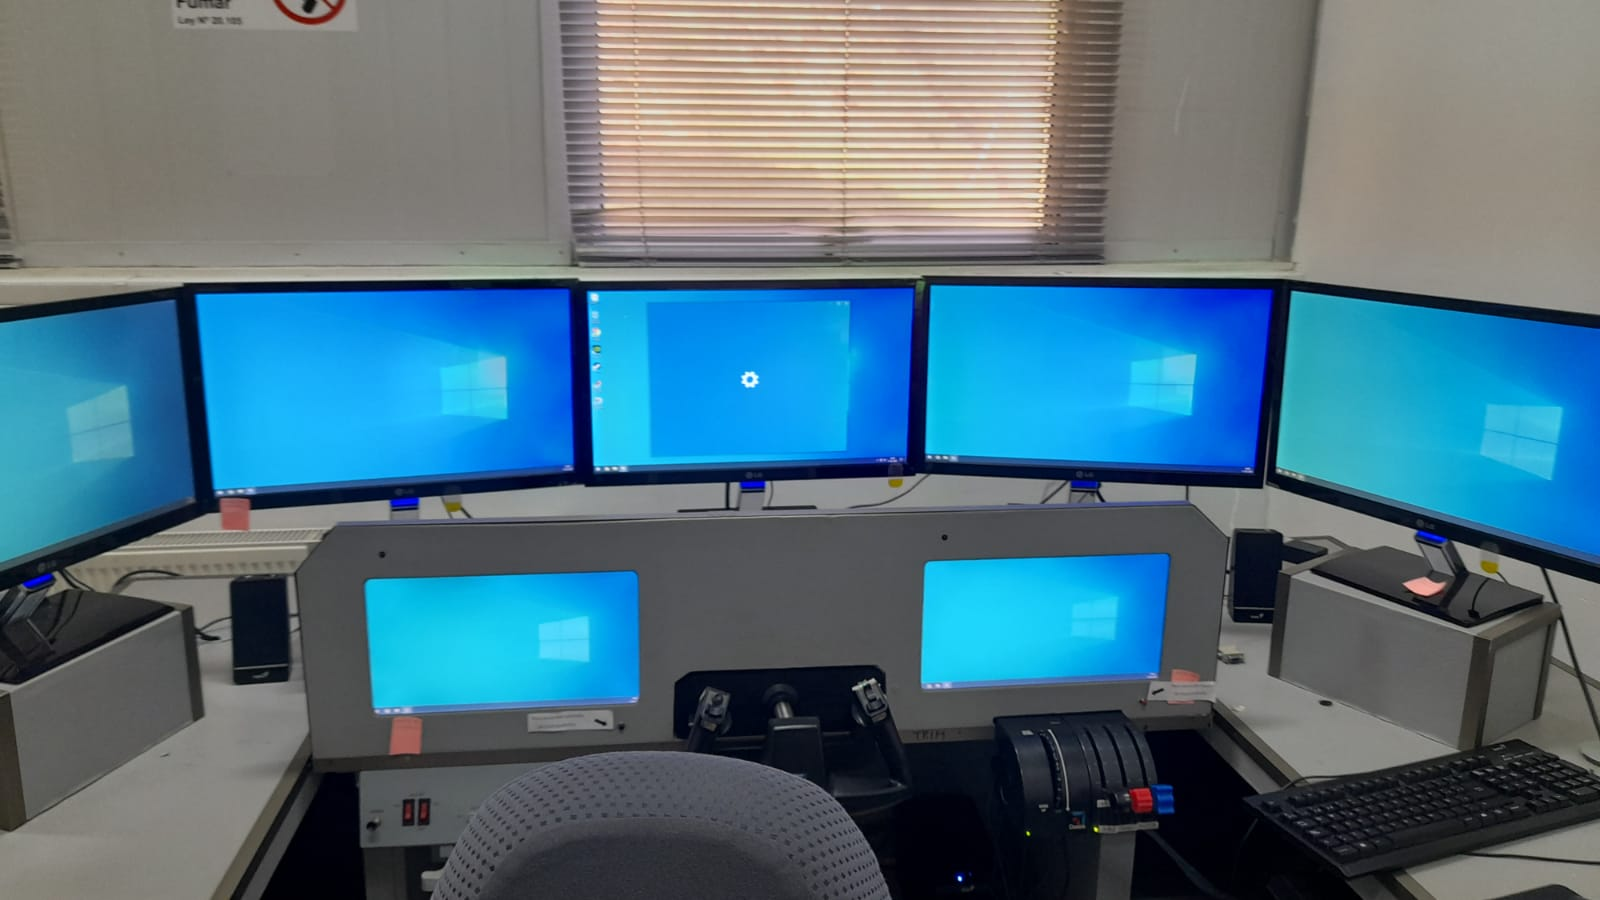
\includegraphics{sim6.jpeg}
	\caption{Simulador de vuelo con configuración final}
	\label{fig:sim6}
\end{figure}

\subsection{Software}

% De que se trata configurar el software
Preparar el software abarca desde formatear el dispositivo de almacenamiento hasta configurar los programas, de tal manera que desde el encendido del equipo se pueda rápidamente empezar una simulación y volar.

% Formateo e instalación de Windows 10 actualizado
Desde los servidores de Microsoft se obtiene la imagen de disco más reciente de Windows 10 \cite{windows}, se graba en un disco duro externo USB y se instala formateando el almacenamiento. Windows se encarga de descargar automáticamente todos los drivers necesarios, incluso el de los periféricos de control.

% Detalles post instalación de windows
Posterior a la instalación, completada la información que se solicite y actualizado el equipo, se ordenan las pantallas en el panel de control de NVIDIA de manera que las 5 pantallas superiores formen una imagen continua y las 2 pantallas auxiliares se desplazan a la parte inferior, con la herramienta de administración de discos de Windows se divide la partición principal creando una nueva partición de 300 GB, con el propósito de almacenar los archivos de instalación del software como respaldo, como por ejemplo las imágenes de disco de X-Plane 9 y 10.

% Descarga de X-Plane 9 desde las carpetas udec en onedrive y respaldo de discos de X-Plane 10
La universidad dispone de copias de X-Plane 9 y X-Plane 10, los archivos de X-Plane 9 se descargan desde una carpeta compartida en OneDrive proporcionada, estos archivos vienen en formato de imágenes de disco MDF y se instala el software WinCDEmu \cite{wincdemu} para poder cargarlas uno a uno. De X-Plane 10 se cuenta con los discos físicos, el computador principal no tiene un lector de DVD por lo que temporalmente se conecta uno de los equipos secundarios que si tiene lector y se crean imágenes de disco con el programa ImgBurn \cite{imgburn}, que luego se copian al principal para completar la instalación de la misma forma que como con X-Plane 9.

% Configuración de multiples X-Plane con script de Autohotkey
[Scripts para ordenar las multiples instancias de X-Plane aún en desarrollo]

\section{Resultados}

A los pocos días de haber terminado la configuración del hardware con múltiples pantallas, los integrantes del simulador de vuelo en el laboratorio de técnicas aeroespaciales realizaron pruebas con versiones de demostración de Flight Simulator 2020 y X-Plane 12 (\ref{fig:sim7}), a pesar de que el rendimiento era bajo los alumnos pudieron configurar los controles y realizar vuelos, incluso invitando a otros alumnos y docentes a pilotar y ver los resultados.

\begin{figure}[h]
	\centering
	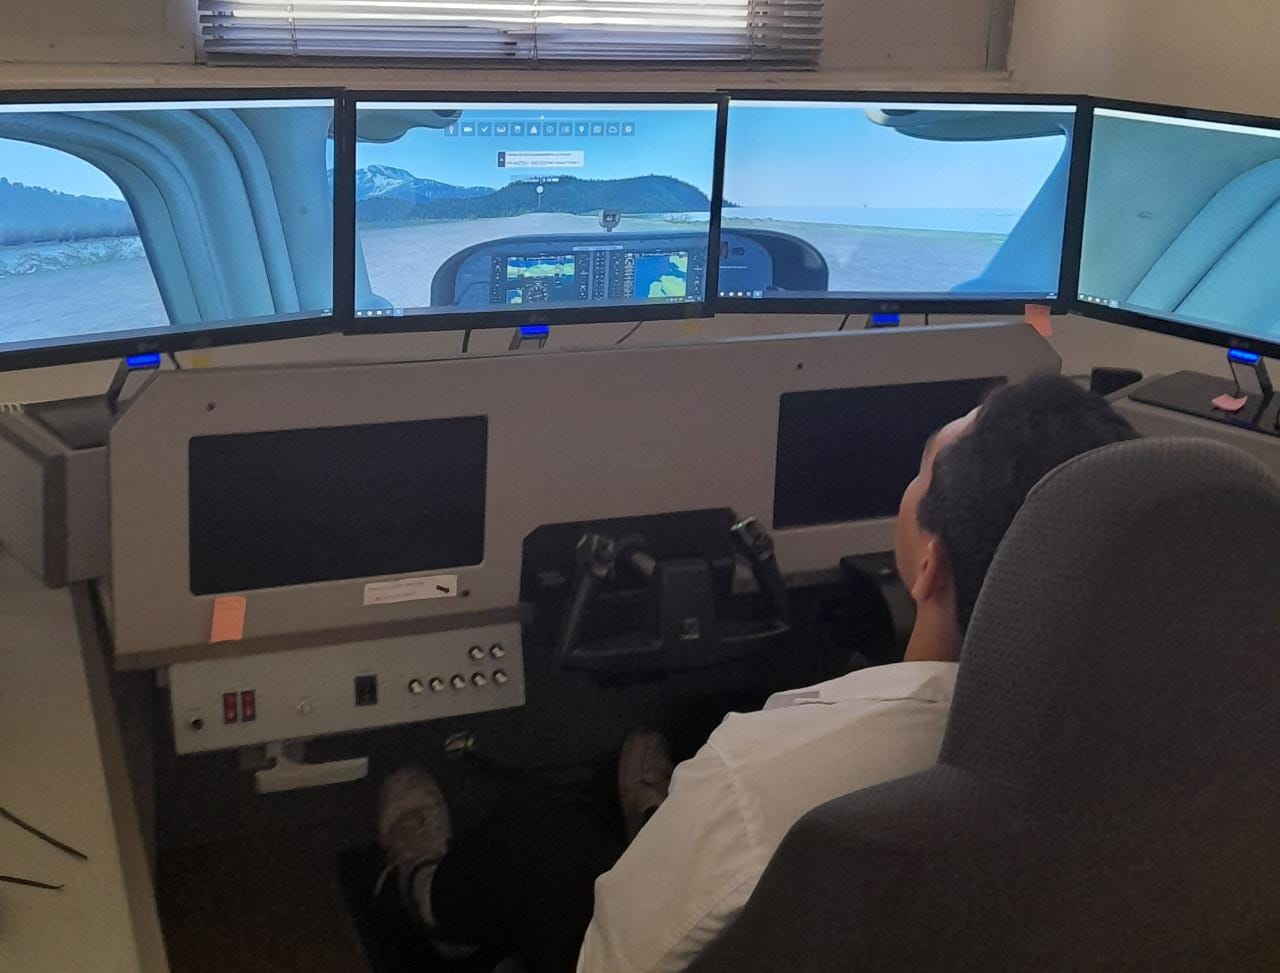
\includegraphics{sim7.jpeg}
	\caption{Pruebas con Microsoft Flight Simulator 2020}
	\label{fig:sim7}
\end{figure}

El software más reciente instalado por los integrantes del grupo de interés incluye soporte para configuración multi-pantalla sin necesidad de trucos como abrir más de una instancia del programa, por lo que fue una tarea fácil configurarlo, sin embargo los simuladores X-Plane antiguos proporcionados por la universidad requieren más trabajo porque la disposición multi-pantalla con un solo computador no está considerada en los manuales \cite{manual9}.

En conclusión se lograron los objetivos, se cumple la solicitud de actualizar el simulador con los nuevos componentes y se simplifica la disposición de tres computadores a solo uno, habilitando un camino claro de actualización que es la compra de nuevas piezas como un procesador más reciente o almacenamiento de estado sólido, se reducen los tiempos necesarios para instalar nuevo software, configurarlo y se asegura un futuro próspero para el grupo de interés del simulador de vuelo.